%!TEX root = bambi-thesis.tex

\chapter{MAVLink Protocol} % (fold)
\label{appendix:mavlink}
\textit{“MAVLink is a very lightweight messaging protocol for communicating with drones (and between onboard drone components).\\
MAVLink follows a modern hybrid publish-subscribe and point-to-point design pattern: Data streams are sent / published as topics while configuration sub-protocols such as the mission protocol or parameter protocol are point-to-point with retransmission.\\
Messages are defined within XML files. Each XML file defines the message set supported by a particular MAVLink system, also referred to as a "dialect". The reference message set that is implemented by most ground control stations and autopilots is defined in common.xml (most dialects build on top of this definition).\\
The MAVLink toolchain uses the XML message definitions to generate MAVLink libraries for each of the supported programming languages. Drones, ground control stations, and other MAVLink systems use the generated libraries to communicate. These are typically MIT-licensed, and can therefore be used without limits in any closed-source application without publishing the source code of the closed-source application.”} \cite{Mavlink}
\paragraph{Key Features} % (fold)
\label{par:key_features}
\begin{itemize}
	\item Very efficient. MAVLink 1 has just 8 bytes overhead per packet, including start sign and packet drop detection. MAVLink 2 has just 14 bytes of overhead (but is a much more secure and extensible protocol). Because MAVLink doesn't require any additional framing it is very well suited for applications with very limited communication bandwidth. 
	\item Very reliable. MAVLink has been used since 2009 to communicate between many different vehicles, ground stations (and other nodes) over varied and challenging communication channels (high latency/noise). It provides methods for detecting packet drops, corruption, and for packet authentication.
	\item Supports many programming languages, running on numerous microcontrollers/operating systems (including ARM7, ATMega, dsPic, STM32 and Windows, Linux, MacOS, Android and iOS).
	\item Allows up to 255 concurrent systems on the network (vehicles, ground stations, etc.)
	\item Enables both offboard and onboard communications (e.g. between a GCS and drone, and between drone autopilot and MAVLink enabled drone camera).
\end{itemize}
In  a second version of the MAVLink protocol was release mainly to allow more then 256 message IDs as it was in the first version. In addition MAVLink 2 is backward-compatible and implement package signing (authentication) which greatly improves security. Basic frame is shown in \autoref{fig:mavlink-packet} and each fields is described in \autoref{tbl:mavlink-frame}. There are several MAVLink messages. Understanding them is vital for sending proper commands to the mav.
\begin{figure}[ht]
    \centering
    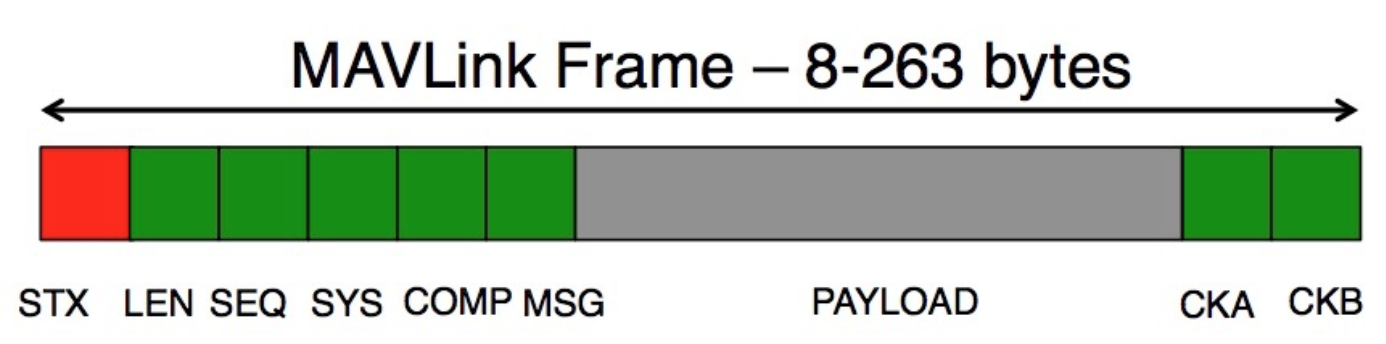
\includegraphics[width=0.6\textwidth]{figures/A2/MAVLink-frame.png}
    \caption{MAVLink packet \cite{MavlinkSerialization}}
    \label{fig:mavlink-packet}
\end{figure}

\begin{table}[ht]
\begin{tabularx}{\textwidth}{|p{1.5cm}|p{3cm}|p{1.8cm}|X|}
\hline
\textbf{Byte Index} 	&\textbf{Content}					   & \textbf{Value}     & \textbf{Description} \\ \hline 
0 						& Start byte of package                & 0xFD         		& Protocol-specific start-of-text (STX) marker used to indicate the beginning of a new packet. Any system that does not understand protocol version will skip the packet. \\  \hline
1                    	& Payload length                       & 0 - 255      		& Indicates length of the following payload section.                                                                                                                      \\  \hline
2                    	& Incompatibility Flags                &              		& Flags that must be understood for MAVLink compatibility (discards packet if it does not understand flag).                                                \\  \hline
3                    	& Compatibility Flags                  &              		& Flags ignored if not understood (implementation handle packet even if it does not understand flag). \\  \hline
4                    	& Packet sequence number               & 0 - 255      		& Used to detect packet loss. Components increment value for each message sent. \\  \hline
5                    	& System ID (sender)                   & 1 - 255      		& ID of system sending the message. Used to differentiate systems on network. \\  \hline
6                   	& Component ID (sender)                & 0 - 255      		& ID of component sending the message. Used to differentiate components in a system (e.g. autopilot and a camera).   \\  \hline
7 to 9               	& Message ID (low, middle, high bytes) & 0 - 16777215 		& ID of message type in payload. Used to decode data back into message object. \\  \hline
10 to (n+10)         	& Payload                              &              		& Message data. Depends on message type (i.e. Message ID) and contents.  \\  \hline
(n+11) to (n+12)     	& Checksum (low byte, high byte)       &              		& X.25 CRC for message (excluding magic byte). Includes CRC\_EXTRA byte. \\  \hline
(n+12) to (n+26)     	& Signature                            &              		& (Optional) Signature to ensure the link is tamper-proof. \\ \hline                                                                           
\end{tabularx}
\caption{Mavlink Packet Field Description \cite{MavlinkSerialization}}
\label{tbl:mavlink-frame}
\end{table}

\paragraph{MAVLink messages\\} % (fold)
\label{par:mavlink_messages}
It follows a short list of the most commonly used MAVLink messages:
\begin{enumerate}
	\item MAVLINK\_MSG\_ID\_REQUEST\_DATA\_STREAM\\ This message is used to request the stream of data from the autopilot. Requested data can be sensors, RC channels, GPS position, status or the combination of them.
	\item MAVLINK\_MSG\_ID\_COMMAND\_LONG\\ This message is used to give commands to the autopilot. Several commands are supported.
	\item SET\_MODE\\ It sets the different mode of operations for the drone. Few supported modes for ArduCopter are	
\end{enumerate}

% paragraph mavlink_messages (end)

% paragraph key_features (end)

% \begin{figure}[ht]
%     \centering
%     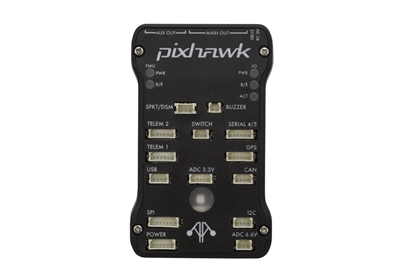
\includegraphics[width=.6\textwidth]{figures/A1/pixhawk.jpg}
%     \caption{}
%     \label{fig:Pixhawk Flight Controller}
% \end{figure}
